
%% bare_conf.tex
%% V1.4b
%% 2015/08/26
%% by Michael Shell
%% See:
%% http://www.michaelshell.org/
%% for current contact information.
%%
%% This is a skeleton file demonstrating the use of IEEEtran.cls
%% (requires IEEEtran.cls version 1.8b or later) with an IEEE
%% conference paper.
%%
%% Support sites:
%% http://www.michaelshell.org/tex/ieeetran/
%% http://www.ctan.org/pkg/ieeetran
%% and
%% http://www.ieee.org/

%%*************************************************************************
%% Legal Notice:
%% This code is offered as-is without any warranty either expressed or
%% implied; without even the implied warranty of MERCHANTABILITY or
%% FITNESS FOR A PARTICULAR PURPOSE! 
%% User assumes all risk.
%% In no event shall the IEEE or any contributor to this code be liable for
%% any damages or losses, including, but not limited to, incidental,
%% consequential, or any other damages, resulting from the use or misuse
%% of any information contained here.
%%
%% All comments are the opinions of their respective authors and are not
%% necessarily endorsed by the IEEE.
%%
%% This work is distributed under the LaTeX Project Public License (LPPL)
%% ( http://www.latex-project.org/ ) version 1.3, and may be freely used,
%% distributed and modified. A copy of the LPPL, version 1.3, is included
%% in the base LaTeX documentation of all distributions of LaTeX released
%% 2003/12/01 or later.
%% Retain all contribution notices and credits.
%% ** Modified files should be clearly indicated as such, including  **
%% ** renaming them and changing author support contact information. **
%%*************************************************************************


% *** Authors should verify (and, if needed, correct) their LaTeX system  ***
% *** with the testflow diagnostic prior to trusting their LaTeX platform ***
% *** with production work. The IEEE's font choices and paper sizes can   ***
% *** trigger bugs that do not appear when using other class files.       ***                          ***
% The testflow support page is at:
% http://www.michaelshell.org/tex/testflow/



\documentclass[conference]{IEEEtran}
\usepackage{amsmath}
\usepackage{graphicx}

% Some Computer Society conferences also require the compsoc mode option,
% but others use the standard conference format.
%
% If IEEEtran.cls has not been installed into the LaTeX system files,
% manually specify the path to it like:
% \documentclass[conference]{../sty/IEEEtran}





% Some very useful LaTeX packages include:
% (uncomment the ones you want to load)


% *** MISC UTILITY PACKAGES ***
%
%\usepackage{ifpdf}
% Heiko Oberdiek's ifpdf.sty is very useful if you need conditional
% compilation based on whether the output is pdf or dvi.
% usage:
% \ifpdf
%   % pdf code
% \else
%   % dvi code
% \fi
% The latest version of ifpdf.sty can be obtained from:
% http://www.ctan.org/pkg/ifpdf
% Also, note that IEEEtran.cls V1.7 and later provides a builtin
% \ifCLASSINFOpdf conditional that works the same way.
% When switching from latex to pdflatex and vice-versa, the compiler may
% have to be run twice to clear warning/error messages.






% *** CITATION PACKAGES ***
%
%\usepackage{cite}
% cite.sty was written by Donald Arseneau
% V1.6 and later of IEEEtran pre-defines the format of the cite.sty package
% \cite{} output to follow that of the IEEE. Loading the cite package will
% result in citation numbers being automatically sorted and properly
% "compressed/ranged". e.g., [1], [9], [2], [7], [5], [6] without using
% cite.sty will become [1], [2], [5]--[7], [9] using cite.sty. cite.sty's
% \cite will automatically add leading space, if needed. Use cite.sty's
% noadjust option (cite.sty V3.8 and later) if you want to turn this off
% such as if a citation ever needs to be enclosed in parenthesis.
% cite.sty is already installed on most LaTeX systems. Be sure and use
% version 5.0 (2009-03-20) and later if using hyperref.sty.
% The latest version can be obtained at:
% http://www.ctan.org/pkg/cite
% The documentation is contained in the cite.sty file itself.






% *** GRAPHICS RELATED PACKAGES ***
%
\ifCLASSINFOpdf
  % \usepackage[pdftex]{graphicx}
  % declare the path(s) where your graphic files are
  % \graphicspath{{../pdf/}{../jpeg/}}
  % and their extensions so you won't have to specify these with
  % every instance of \includegraphics
  % \DeclareGraphicsExtensions{.pdf,.jpeg,.png}
\else
  % or other class option (dvipsone, dvipdf, if not using dvips). graphicx
  % will default to the driver specified in the system graphics.cfg if no
  % driver is specified.
  % \usepackage[dvips]{graphicx}
  % declare the path(s) where your graphic files are
  % \graphicspath{{../eps/}}
  % and their extensions so you won't have to specify these with
  % every instance of \includegraphics
  % \DeclareGraphicsExtensions{.eps}
\fi
% graphicx was written by David Carlisle and Sebastian Rahtz. It is
% required if you want graphics, photos, etc. graphicx.sty is already
% installed on most LaTeX systems. The latest version and documentation
% can be obtained at: 
% http://www.ctan.org/pkg/graphicx
% Another good source of documentation is "Using Imported Graphics in
% LaTeX2e" by Keith Reckdahl which can be found at:
% http://www.ctan.org/pkg/epslatex
%
% latex, and pdflatex in dvi mode, support graphics in encapsulated
% postscript (.eps) format. pdflatex in pdf mode supports graphics
% in .pdf, .jpeg, .png and .mps (metapost) formats. Users should ensure
% that all non-photo figures use a vector format (.eps, .pdf, .mps) and
% not a bitmapped formats (.jpeg, .png). The IEEE frowns on bitmapped formats
% which can result in "jaggedy"/blurry rendering of lines and letters as
% well as large increases in file sizes.
%
% You can find documentation about the pdfTeX application at:
% http://www.tug.org/applications/pdftex





% *** MATH PACKAGES ***
%
%\usepackage{amsmath}
% A popular package from the American Mathematical Society that provides
% many useful and powerful commands for dealing with mathematics.
%
% Note that the amsmath package sets \interdisplaylinepenalty to 10000
% thus preventing page breaks from occurring within multiline equations. Use:
%\interdisplaylinepenalty=2500
% after loading amsmath to restore such page breaks as IEEEtran.cls normally
% does. amsmath.sty is already installed on most LaTeX systems. The latest
% version and documentation can be obtained at:
% http://www.ctan.org/pkg/amsmath





% *** SPECIALIZED LIST PACKAGES ***
%
%\usepackage{algorithmic}
% algorithmic.sty was written by Peter Williams and Rogerio Brito.
% This package provides an algorithmic environment fo describing algorithms.
% You can use the algorithmic environment in-text or within a figure
% environment to provide for a floating algorithm. Do NOT use the algorithm
% floating environment provided by algorithm.sty (by the same authors) or
% algorithm2e.sty (by Christophe Fiorio) as the IEEE does not use dedicated
% algorithm float types and packages that provide these will not provide
% correct IEEE style captions. The latest version and documentation of
% algorithmic.sty can be obtained at:
% http://www.ctan.org/pkg/algorithms
% Also of interest may be the (relatively newer and more customizable)
% algorithmicx.sty package by Szasz Janos:
% http://www.ctan.org/pkg/algorithmicx




% *** ALIGNMENT PACKAGES ***
%
%\usepackage{array}
% Frank Mittelbach's and David Carlisle's array.sty patches and improves
% the standard LaTeX2e array and tabular environments to provide better
% appearance and additional user controls. As the default LaTeX2e table
% generation code is lacking to the point of almost being broken with
% respect to the quality of the end results, all users are strongly
% advised to use an enhanced (at the very least that provided by array.sty)
% set of table tools. array.sty is already installed on most systems. The
% latest version and documentation can be obtained at:
% http://www.ctan.org/pkg/array


% IEEEtran contains the IEEEeqnarray family of commands that can be used to
% generate multiline equations as well as matrices, tables, etc., of high
% quality.




% *** SUBFIGURE PACKAGES ***
%\ifCLASSOPTIONcompsoc
%  \usepackage[caption=false,font=normalsize,labelfont=sf,textfont=sf]{subfig}
%\else
%  \usepackage[caption=false,font=footnotesize]{subfig}
%\fi
% subfig.sty, written by Steven Douglas Cochran, is the modern replacement
% for subfigure.sty, the latter of which is no longer maintained and is
% incompatible with some LaTeX packages including fixltx2e. However,
% subfig.sty requires and automatically loads Axel Sommerfeldt's caption.sty
% which will override IEEEtran.cls' handling of captions and this will result
% in non-IEEE style figure/table captions. To prevent this problem, be sure
% and invoke subfig.sty's "caption=false" package option (available since
% subfig.sty version 1.3, 2005/06/28) as this is will preserve IEEEtran.cls
% handling of captions.
% Note that the Computer Society format requires a larger sans serif font
% than the serif footnote size font used in traditional IEEE formatting
% and thus the need to invoke different subfig.sty package options depending
% on whether compsoc mode has been enabled.
%
% The latest version and documentation of subfig.sty can be obtained at:
% http://www.ctan.org/pkg/subfig




% *** FLOAT PACKAGES ***
%
%\usepackage{fixltx2e}
% fixltx2e, the successor to the earlier fix2col.sty, was written by
% Frank Mittelbach and David Carlisle. This package corrects a few problems
% in the LaTeX2e kernel, the most notable of which is that in current
% LaTeX2e releases, the ordering of single and double column floats is not
% guaranteed to be preserved. Thus, an unpatched LaTeX2e can allow a
% single column figure to be placed prior to an earlier double column
% figure.
% Be aware that LaTeX2e kernels dated 2015 and later have fixltx2e.sty's
% corrections already built into the system in which case a warning will
% be issued if an attempt is made to load fixltx2e.sty as it is no longer
% needed.
% The latest version and documentation can be found at:
% http://www.ctan.org/pkg/fixltx2e


%\usepackage{stfloats}
% stfloats.sty was written by Sigitas Tolusis. This package gives LaTeX2e
% the ability to do double column floats at the bottom of the page as well
% as the top. (e.g., "\begin{figure*}[!b]" is not normally possible in
% LaTeX2e). It also provides a command:
%\fnbelowfloat
% to enable the placement of footnotes below bottom floats (the standard
% LaTeX2e kernel puts them above bottom floats). This is an invasive package
% which rewrites many portions of the LaTeX2e float routines. It may not work
% with other packages that modify the LaTeX2e float routines. The latest
% version and documentation can be obtained at:
% http://www.ctan.org/pkg/stfloats
% Do not use the stfloats baselinefloat ability as the IEEE does not allow
% \baselineskip to stretch. Authors submitting work to the IEEE should note
% that the IEEE rarely uses double column equations and that authors should try
% to avoid such use. Do not be tempted to use the cuted.sty or midfloat.sty
% packages (also by Sigitas Tolusis) as the IEEE does not format its papers in
% such ways.
% Do not attempt to use stfloats with fixltx2e as they are incompatible.
% Instead, use Morten Hogholm'a dblfloatfix which combines the features
% of both fixltx2e and stfloats:
%
% \usepackage{dblfloatfix}
% The latest version can be found at:
% http://www.ctan.org/pkg/dblfloatfix




% *** PDF, URL AND HYPERLINK PACKAGES ***
%
%\usepackage{url}
% url.sty was written by Donald Arseneau. It provides better support for
% handling and breaking URLs. url.sty is already installed on most LaTeX
% systems. The latest version and documentation can be obtained at:
% http://www.ctan.org/pkg/url
% Basically, \url{my_url_here}.




% *** Do not adjust lengths that control margins, column widths, etc. ***
% *** Do not use packages that alter fonts (such as pslatex).         ***
% There should be no need to do such things with IEEEtran.cls V1.6 and later.
% (Unless specifically asked to do so by the journal or conference you plan
% to submit to, of course. )


% correct bad hyphenation here
\hyphenation{op-tical net-works semi-conduc-tor}


\begin{document}
%
% paper title
% Titles are generally capitalized except for words such as a, an, and, as,
% at, but, by, for, in, nor, of, on, or, the, to and up, which are usually
% not capitalized unless they are the first or last word of the title.
% Linebreaks \\ can be used within to get better formatting as desired.
% Do not put math or special symbols in the title.
\title{Unsupervised Learning}


% author names and affiliations
% use a multiple column layout for up to three different
% affiliations
\author{\IEEEauthorblockN{Nasrul Huda}
\IEEEauthorblockA{Department of Informatics\\
University of Hamburg, Germany\\
Email: nasrul.huda@studium.uni-hamburg.de }
\and
\IEEEauthorblockN{Laiba Qureshi}
\IEEEauthorblockA{Department of Informatics\\
University of Hamburg, Germany\\
Email: laiba.qureshi@studium.uni-hamburg.de}}
% \and
% \IEEEauthorblockN{James Kirk\\ and Montgomery Scott}
% \IEEEauthorblockA{Starfleet Academy\\
% San Francisco, California 96678--2391\\
% Telephone: (800) 555--1212\\
% Fax: (888) 555--1212}}

% conference papers do not typically use \thanks and this command
% is locked out in conference mode. If really needed, such as for
% the acknowledgment of grants, issue a \IEEEoverridecommandlockouts
% after \documentclass

% for over three affiliations, or if they all won't fit within the width
% of the page, use this alternative format:
% 
%\author{\IEEEauthorblockN{Michael Shell\IEEEauthorrefmark{1},
%Homer Simpson\IEEEauthorrefmark{2},
%James Kirk\IEEEauthorrefmark{3}, 
%Montgomery Scott\IEEEauthorrefmark{3} and
%Eldon Tyrell\IEEEauthorrefmark{4}}
%\IEEEauthorblockA{\IEEEauthorrefmark{1}School of Electrical and Computer Engineering\\
%Georgia Institute of Technology,
%Atlanta, Georgia 30332--0250\\ Email: see http://www.michaelshell.org/contact.html}
%\IEEEauthorblockA{\IEEEauthorrefmark{2}Twentieth Century Fox, Springfield, USA\\
%Email: homer@thesimpsons.com}
%\IEEEauthorblockA{\IEEEauthorrefmark{3}Starfleet Academy, San Francisco, California 96678-2391\\
%Telephone: (800) 555--1212, Fax: (888) 555--1212}
%\IEEEauthorblockA{\IEEEauthorrefmark{4}Tyrell Inc., 123 Replicant Street, Los Angeles, California 90210--4321}}




% use for special paper notices
%\IEEEspecialpapernotice{(Invited Paper)}




% make the title area
\maketitle

% As a general rule, do not put math, special symbols or citations
% in the abstract
\begin{abstract}
% This paper surveys key methods in unsupervised learning, a core machine learning paradigm that enables pattern discovery and representation learning without labeled data. We provide a comparative overview of unsupervised techniques by covering the major categories such as dimensionality reduction, clustering, and association rule learning, presenting the core algorithms, theoretical foundations, strengths and limitations, and practical use cases.  This work aims to offer a comprehensive entry point for understanding the landscape of unsupervised learning methods and their applications.

This paper presents an overview of foundational techniques in unsupervised learning, a central machine learning approach focused on uncovering patterns and representations from unlabeled data. It explores major categories—including dimensionality reduction, clustering, and association rule learning—by outlining fundamental algorithms, underlying theory, practical applications, and the advantages and limitations of each method. The goal is to to offer a comprehensive entry point for understanding the landscape of unsupervised learning methods and their applications.
\end{abstract}

% no keywords




% For peer review papers, you can put extra information on the cover
% page as needed:
% \ifCLASSOPTIONpeerreview
% \begin{center} \bfseries EDICS Category: 3-BBND \end{center}
% \fi
%
% For peerreview papers, this IEEEtran command inserts a page break and
% creates the second title. It will be ignored for other modes.
\IEEEpeerreviewmaketitle



\section{Introduction}
For decades, researchers have explored techniques to harness the vast quantities of unlabeled data available in real-world applications. As noted by Xiaojin Zhu, ``labels are hard to obtain while unlabeled data are abundant" \cite{intro-article}. In an era of rapidly increasing data volumes, manual annotation remains a significant bottleneck. This reinforces the importance of unsupervised learning as a powerful framework for uncovering structure, identifying patterns, and generating insights directly from raw data—without the need for labeled examples. \\

Unsupervised methods have become essential in domains where labeled data is unavailable or expensive to obtain. They are particularly useful in exploratory analysis, anomaly detection, and scenarios where human labeling is infeasible, such as genomics, recommender systems, and social network analysis \cite{socialmedia, gene}. \\

% \textbf{can add more in intro if space left (like generative)!}
In recent years, generative models have made significant advances in unsupervised learning. By learning to generate data that resembles the input distribution, models such as Variational Autoencoders (VAEs) and Generative Adversarial Networks (GANs) uncover meaningful latent structures, enabling tasks like representation learning, synthetic data generation, clustering, and data compression \cite{generative}.

\subsection{Report Overview}
This report provides a comprehensive overview of key methods in unsupervised learning. It begins by contrasting the three main machine learning paradigms—supervised, unsupervised, and reinforcement learning—highlighting their core objectives and differences. The focus then shifts to major categories within unsupervised learning, namely \textit{\textbf{Dimensionality Reduction}}, \textit{\textbf{Clustering}}, and \textit{\textbf{Association Rule Learning}}. For each category, we present widely used algorithms, discuss their underlying principles and mathematical formulations, evaluate their strengths and limitations, and explore real-world applications where these methods are effectively employed.

%The report also includes additional methodological insights and elaborations that extend beyond the original presentation.

% practical use cases and additional methodological insights that extend beyond the scope of the accompanying presentation.


% \hfill mds
 
% \hfill August 26, 2015

% \subsection{Subsection Heading Here}
% Subsection text here.


% \subsubsection{Subsubsection Heading Here}
% Subsubsection text here.


\section{The Three Learning Rules}
Machine learning is commonly categorized into three main paradigms based on the nature of the data and the learning objective \cite{unsupervised}: 

\subsection{Reinforcement Learning}
Reinforcement learning involves an agent that interacts with an environment and learns to make decisions by receiving rewards or penalties. The objective is to learn a policy that maximizes cumulative reward over time. Key algorithms include Q-learning, Deep Q Networks (DQN), and policy gradient methods. Reinforcement learning has been successfully applied in fields such as robotics, autonomous driving, and game playing (e.g., AlphaGo) \cite{Hui_2018}.

\subsection{Supervised Learning}
Supervised learning involves learning a function that maps inputs to outputs based on labeled data. The goal is typically predictive—either classification or regression. Popular algorithms include linear regression, logistic regression, support vector machines (SVMs), decision trees, and neural networks \cite{supervised}. Example use cases include spam detection, image classification, and medical diagnosis.

\subsection{Unsupervised Learning}
Unsupervised learning refers to a class of techniques aimed at identifying patterns or structures in datasets without predefined labels \cite{unsupervised}. Unlike supervised learning, which relies on input-output pairs, unsupervised learning algorithms operate on unlabeled data, discovering groupings, correlations, or lower-dimensional representations on their own. These models learn to organize data by detecting similarities and differences, often revealing hidden structures that may not be evident through manual analysis. Common techniques include k-means clustering, DBSCAN, hierarchical clustering, Apriori algorithm, principal component analysis (PCA), and t-SNE, all of which are explained in detail below. 
% The overarching goal is to uncover meaningful insights or features from data without external supervision, making it valuable for exploratory data analysis and preprocessing in more complex pipelines.

\section{Dimensionality Reduction}
Dimensionality reduction is a technique that reduces the number of features or dimensions in a dataset by creating a smaller set of new variables that retain the essential information. It is is widely used both for facilitating data visualization and as a pre-processing step to improve the performance of supervised learning algorithms.
\subsection{Principal Component Analysis (PCA)}
In many real-world datasets, features may be highly correlated, making analysis redundant and visualization difficult in high-dimensional space. Principal Component Analysis (PCA) mitigates this challenge by identifying a lower-dimensional representation of the the original correlated variables into into a smaller set of uncorrelated variables, called principal components, that captures the maximum possible variance in the data, thereby facilitating more efficient analysis and visualization. \\
% Given a dataset with n and p features, examining all pairwise scatterplots to uncover underlying structure becomes increasingly impractical as the dimensionality `p' grows. Principal Component Analysis (PCA) mitigates this challenge by identifying a lower-dimensional representation that captures the maximum possible variance in the data, thereby facilitating more efficient analysis and visualization. \\

PCA is not only useful in data summarization and compression, but also in handling missing values through imputation and for pre-processing the data for any supervised learning model. 

\subsubsection{Mathematical Formulation}

Let \( \mathbf{X} \) be a dataset with \( n \) observations and \( p \) features. We assume that the data is \textit{centered}, i.e., the mean of each feature (column) has been subtracted so that:

\[
\frac{1}{n} \sum_{i=1}^{n} x_{ij} = 0 \quad \text{for all } j = 1, \dots, p
\]

The first principal component is defined as a normalized linear combination of the original features \cite{James2021}:

\[
Z_1 = \phi_{11}X_1 + \phi_{21}X_2 + \cdots + \phi_{p1}X_p
\]

or more compactly:

\[
Z_1 = \boldsymbol{\phi}_1^{\top} \mathbf{X}
\]

where \( \boldsymbol{\phi}_1 = (\phi_{11}, \phi_{21}, \dots, \phi_{p1})^{\top} \) is the \textit{loading vector} for the first principal component. The loadings are subject to the constraint \cite{James2021}:

\[
\sum_{j=1}^{p} \phi_{j1}^2 = 1
\]

This normalization ensures that the variance of the principal component cannot be made arbitrarily large by scaling the loadings.

Each observation \( \mathbf{x}_i = (x_{i1}, x_{i2}, \dots, x_{ip}) \) is projected onto the principal component axis as:

\[
z_{i1} = \phi_{11} x_{i1} + \phi_{21} x_{i2} + \cdots + \phi_{p1} x_{ip}
\]

The resulting values \( z_{i1} \) are referred to as the \textit{scores} of the first principal component.

The goal is to find the loading vector that maximizes the sample variance of the scores \cite{James2021}:

\[
\underset{\phi_{11}, \dots, \phi_{p1}}{\text{maximize}} \left\{ \frac{1}{n} \sum_{i=1}^{n} \left( \sum_{j=1}^{p} \phi_{j1} x_{ij} \right)^2 \right\} \quad \text{subject to } \sum_{j=1}^{p} \phi_{j1}^2 = 1
\]

This optimization problem can be solved via \textit{eigenvalue decomposition} of the sample covariance matrix:

\[
\mathbf{S} = \frac{1}{n} \mathbf{X}^{\top} \mathbf{X}
\]

The solution yields:
\begin{itemize}
  \item \textbf{Eigenvectors:} These correspond to the loading vectors \( \boldsymbol{\phi}_1, \boldsymbol{\phi}_2, \dots \)
  \item \textbf{Eigenvalues:} These represent the amount of variance explained by each corresponding principal component
\end{itemize} 
\vspace{0.5em}
The first principal component corresponds to the eigenvector associated with the largest eigenvalue, as it captures the greatest variance in the data. Subsequent principal components (e.g., \( Z_2, Z_3, \dots \)) are derived similarly, with the additional constraint of being orthogonal (i.e., uncorrelated) to the previously computed components. \\

\subsubsection{Choosing Appropriate Components}
To determine an appropriate number of principal components \( k \), one typically analyzes the proportion of variance each component explains. Let \( \lambda_1, \lambda_2, \dots, \lambda_p \) be the eigenvalues of the covariance matrix, ordered in decreasing magnitude. The cumulative proportion of variance explained by the first \( k \) components is given by:

\[
\text{Explained Variance Ratio (EVR)} = \frac{\sum_{i=1}^{k} \lambda_i}{\sum_{i=1}^{p} \lambda_i}
\]

A common heuristic is to choose the smallest \( k \) such that the EVR exceeds a threshold—typically 90\% or 95\%—ensuring that the reduced dimensionality retains most of the original information. This decision is often aided by examining a \textit{scree plot}, which visualizes the eigenvalues in descending order. The ``elbow" point in this plot, where the marginal gain in explained variance drops off significantly, suggests a natural cutoff for selecting \( k \) (see Fig.~\ref{fig:scree}).

\begin{figure}[h]
\centering
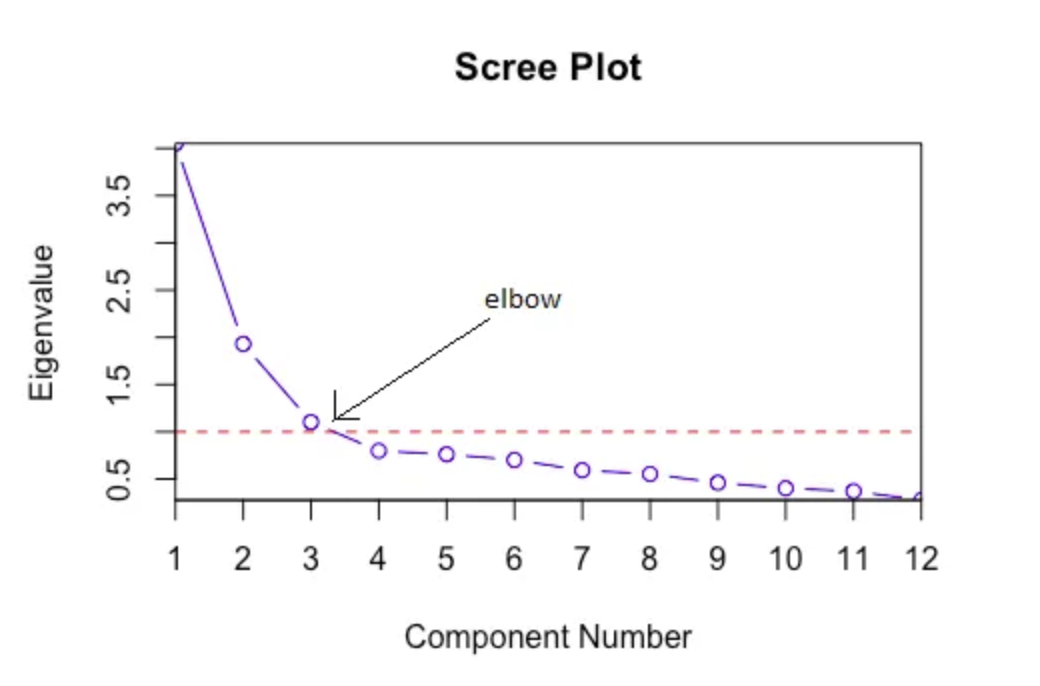
\includegraphics[width=0.5\textwidth]{scree_plot.png}
\caption{Example scree plot for selecting the number of principal components \cite{screeplot}.}
\label{fig:scree}
\end{figure}
\subsection{t-distributed Stochastic Neighbor Embedding (t-SNE)}
t-Distributed Stochastic Neighbor Embedding (t-SNE), introduced by van der Maaten and Hinton (2008), is a nonlinear dimensionality reduction technique designed to visualize high-dimensional data in a lower-dimensional space (typically 2D or 3D) \cite{tsne}. t-SNE focuses on maintaining the \emph{local structure} of the data — that is, ensuring that data points that are close together in the high-dimensional space remain close in the low-dimensional embedding. \\

The core idea of t-SNE is to minimize the mismatch between two probability distributions:
\begin{itemize}
    \item A distribution \( P \) that captures pairwise similarities between points in the high-dimensional space.
    \item A distribution \( Q \) that reflects those similarities in the lower-dimensional embedding.
\end{itemize} 
\vspace{0.5em}
\paragraph{High-dimensional similarity} The similarity between two points \( x_i \) and \( x_j \) in the original space is modeled as a conditional probability \( p_{j|i} \) in proportion to the probability density under a Gaussian centered at \( x_i \) \cite{tsne}:

\[
p_{j|i} = \frac{\exp(-\|x_i - x_j\|^2 / 2\sigma_i^2)}{\sum_{k \neq i} \exp(-\|x_i - x_k\|^2 / 2\sigma_i^2)}
\]

\paragraph{Low-dimensional similarity} In the embedding space, the similarity \( q_{ij} \) between two points \( y_i \) and \( y_j \) is modeled using a Student's t-distribution with one degree of freedom (equivalent to the Cauchy distribution) \cite{tsne}:

\[
q_{ij} = \frac{(1 + \|y_i - y_j\|^2)^{-1}}{\sum_{k \neq l} (1 + \|y_k - y_l\|^2)^{-1}}
\]

The use of the t-distribution, with its heavier tails compared to the Gaussian, helps prevent the \textit{crowding problem}, where distant points in the high-dimensional space are erroneously mapped too close together in the low-dimensional space. \\

Rather than computing separate conditional probabilities \( p_{j|i} \) and \( q_{j|i} \), t-SNE defines joint probabilities:

\[
p_{ij} = \frac{p_{j|i} + p_{i|j}}{2n}, \quad q_{ij} = \frac{(1 + \|\mathbf{y}_i - \mathbf{y}_j\|^2)^{-1}}{\sum_{k \neq l} (1 + \|\mathbf{y}_k - \mathbf{y}_l\|^2)^{-1}}
\]

This leads to a single cost function based on the Kullback-Leibler (KL) divergence which t-SNE uses to minimize the divergence between the high-dimensional and low-dimensional distributions \cite{tsne}:

\[
C = KL(P \| Q) = \sum_{i} \sum_{j} p_{ij} \log \left( \frac{p_{ij}}{q_{ij}} \right)
\]

% The gradient of this cost with respect to the low-dimensional embedding \( \mathbf{y}_i \) is:

% \[
% \frac{\partial C}{\partial \mathbf{y}_i} = 4 \sum_{j} (p_{ij} - q_{ij})(\mathbf{y}_i - \mathbf{y}_j)
% \]
% t-SNE minimizes the divergence between the high-dimensional and low-dimensional distributions using the Kullback–Leibler (KL) divergence.

This cost function is minimized using gradient descent. The gradient of the KL divergence with respect to a low-dimensional point \( y_i \) guides the optimization: for each pair \( (i, j) \), if \( p_{ij} > q_{ij} \), then \( y_i \) and \( y_j \) are pulled closer together; otherwise, they are pushed apart.


\subsection{Additional approaches}
In addition to PCA and t-SNE, several other dimensionality reduction techniques are widely used, each with its own strengths. \textit{Uniform Manifold Approximation and Projection (UMAP)} is a recent method that, like t-SNE, preserves local structure but also maintains more of the global relationships \cite{umap}. It is often faster and more scalable for large datasets. \textit{Isomap} and \textit{Locally Linear Embedding (LLE)} are manifold learning techniques that aim to capture the intrinsic geometry of nonlinear data by preserving geodesic or local linear relationships \cite{isomap, LLE}. Another powerful family of methods are \textit{Autoencoders}, which are neural network-based architectures that learn compact, meaningful representations by training the network to reconstruct its input \cite{autoencoder}. These nonlinear techniques are particularly useful when working with complex or high-dimensional datasets where linear methods fall short. 


\section{Clustering}
Clustering is an unsupervised machine learning technique that partitions a dataset into groups, or clusters, such that observations within the same cluster exhibit high similarity, while those in different clusters are dissimilar. It is widely used to uncover hidden patterns or intrinsic structures in data without relying on labeled outcomes. %Applications of clustering span various fields, including market segmentation, biological data analysis, and image processing.
\subsection{k-Means Clustering}
K-means clustering is a centroid-based method for partitioning a dataset into \( K \) distinct, non-overlapping clusters \cite{ikotun2023kmeans}. It assumes that the desired number of clusters \( K \) is known in advance \cite{clusters}. Each data point is assigned to the cluster with the nearest mean (centroid), and the centroids are iteratively updated to minimize the total within-cluster variation. \\

Formally, let \( C_1, C_2, \ldots, C_K \) be the clusters, where each \( C_k \) contains indices of the observations assigned to the \( k \)-th cluster. The objective of K-means is to minimize the total within-cluster variation \cite{James2021}:

\[
\min_{C_1, \ldots, C_K} \sum_{k=1}^K W(C_k)
\]

where the within-cluster variation \( W(C_k) \) is typically defined using the squared Euclidean distance :

\[
W(C_k) = \frac{1}{|C_k|} \sum_{i, i' \in C_k} \sum_{j=1}^p (x_{ij} - x_{i'j})^2
\]

This leads to the overall optimization problem \cite{James2021}:

\[
\min_{C_1, \ldots, C_K} \sum_{k=1}^K \frac{1}{|C_k|} \sum_{i, i' \in C_k} \sum_{j=1}^p (x_{ij} - x_{i'j})^2
\]

A more computationally efficient formulation uses the cluster mean \( \bar{x}_{kj} \) for each feature \( j \) in cluster \( C_k \):

\[
W(C_k) = 2 \sum_{i \in C_k} \sum_{j=1}^p (x_{ij} - \bar{x}_{kj})^2
\]

\paragraph{Algorithm}
The standard K-means algorithm works as follows:

\begin{enumerate}
    \item Randomly assign each data point to one of the \( K \) clusters.
    \item Repeat until convergence:
        \begin{enumerate}
            \item Compute the centroid of each cluster.
            \item Reassign each data point to the cluster with the nearest centroid.
        \end{enumerate}
\end{enumerate}

This iterative approach guarantees that the objective function never increases and eventually converges to a local minimum. However, because the solution is sensitive to initialization, it is common practice to run K-means multiple times with different random seeds and select the best outcome based on the lowest objective value. \\

\subsubsection{Optimal value of K}
Selecting the appropriate value of \( K \) in K-means clustering is crucial, as it directly impacts the quality and interpretability of the clustering. Two commonly used methods: \\

\textbf{Elbow Method:} This method involves plotting the total within-cluster sum of squares (WCSS) against different values of \( K \). Initially, WCSS decreases sharply as \( K \) increases, but after a certain point, the rate of decrease slows—forming an ``elbow". This elbow indicates the optimal number of clusters, as shown in Fig.~\ref{fig:elbow} below.

\begin{figure}[h]
    \centering
    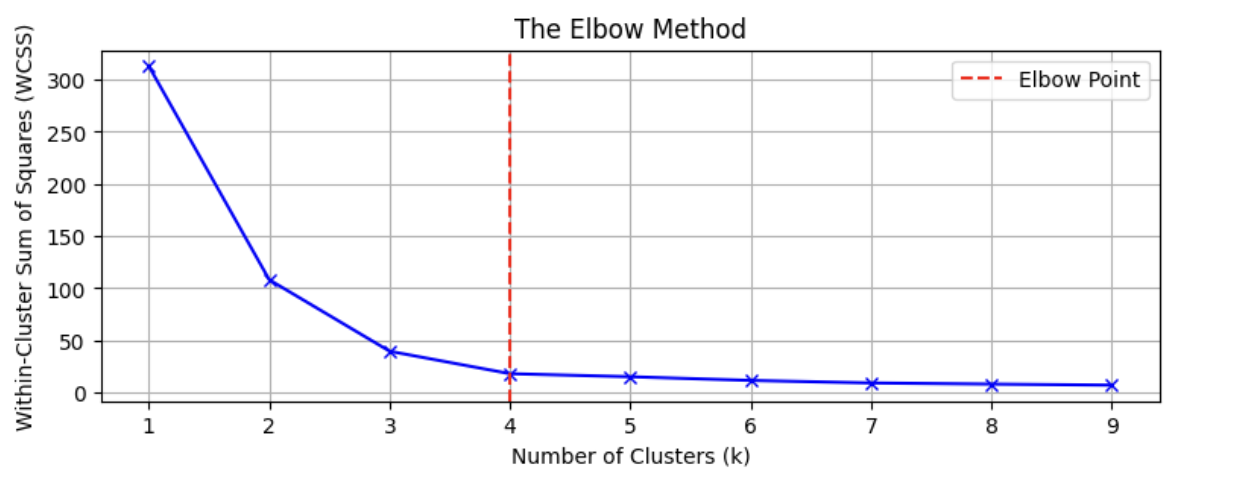
\includegraphics[width=0.5\textwidth]{elbow_method.png}
    \caption{Elbow method showing distortion score vs. number of clusters \cite{geeksforgeeks_elbow}.}
    \label{fig:elbow}
\end{figure}

\textbf{Silhouette Score:} This metric evaluates the quality of clustering by measuring how similar a point is to its own cluster compared to other clusters. It ranges from \(-1\) to \(1\), where a higher value indicates better-defined and well-separated clusters. The optimal \( K \) is the one with the highest average silhouette score. (Fig.~\ref{fig:silhouette})

\begin{figure}[h]
    \centering
    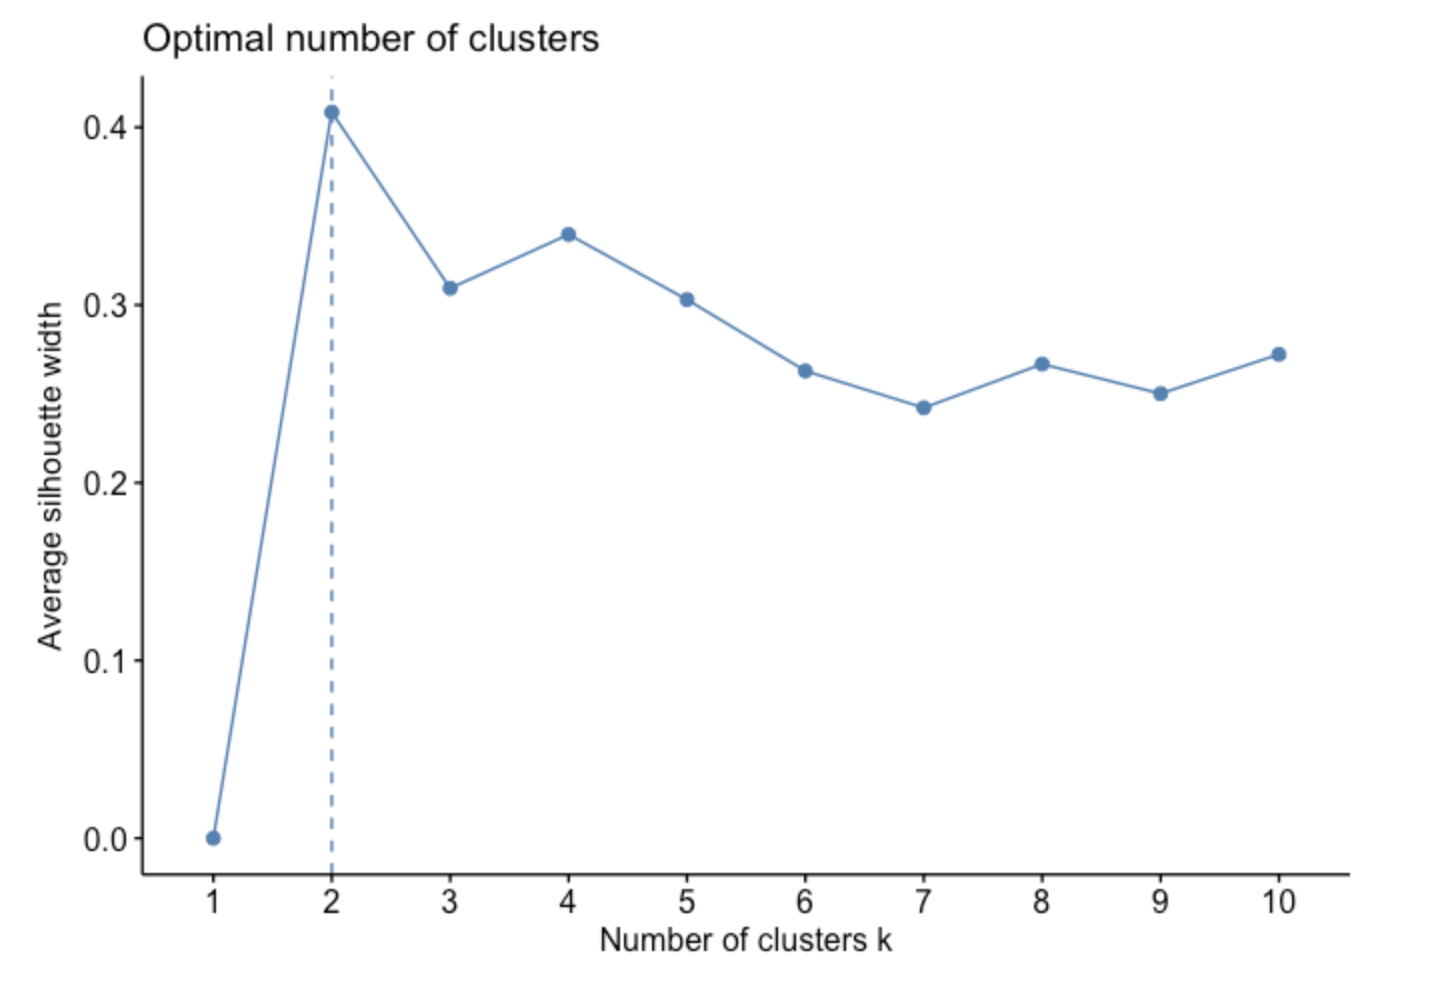
\includegraphics[width=0.5\textwidth]{silhouette_example.png}
    \caption{Avg silhouette scores for different values of \( K \). Highest score indicates optimal cluster count \cite{uc_r_kmeans}.}
    \label{fig:silhouette}
\end{figure}

Both methods provide heuristic guidelines, and often they are used together or supported with domain knowledge to make a final decision about the number of clusters.

\subsection{Hierarchical Clustering}
Hierarchical Clustering is a tree representation of clusters of a given dataset. Leaves of the tree represent individual data points and each internal node defines a cluster on leaf nodes of its descendants. It is used to group similar data points together based on their similarity creating hierarchy or tree-like structure. Hierarchical clustering does not require a prespecified number of clusters. Hierarchical Clustering algorithms fall into two classes - agglomerative hierarchical clustering and divisive clustering \cite{manning2008information, tan2005clustering}. \\

\textbf{Agglomerative Clustering:} Also known as the bottom-up approach. In Hierarchical Agglomerative Clustering(HAC), the key idea is to begin with each data point and treat them as their own individual clusters and then start merging the nodes or clusters recursively based on their similarity measure.\\

An HAC clustering is typically visualised as a dendrogram as shown in Fig.~\ref{fig:dendrogram}. Each merge is represented by a horizontal line. The y-coordinate of the horizontal line is the similarity of the two clusters that were merged, where documents are viewed as singleton clusters. We call this similarity the \textit{combination similarity} of the merged cluster. For example, the combination similarity of the cluster consisting of \textit{Lloyd's CEO questioned} and \textit{Lloyd's chief / U.S. grilling} in the figure~\ref{fig:dendrogram} $\approx$ 0.56. We define the combination similarity of a singleton cluster as its document's self-similarity (which is 1.0 for cosine similarity). \\

\begin{figure}[h]
  \centering
  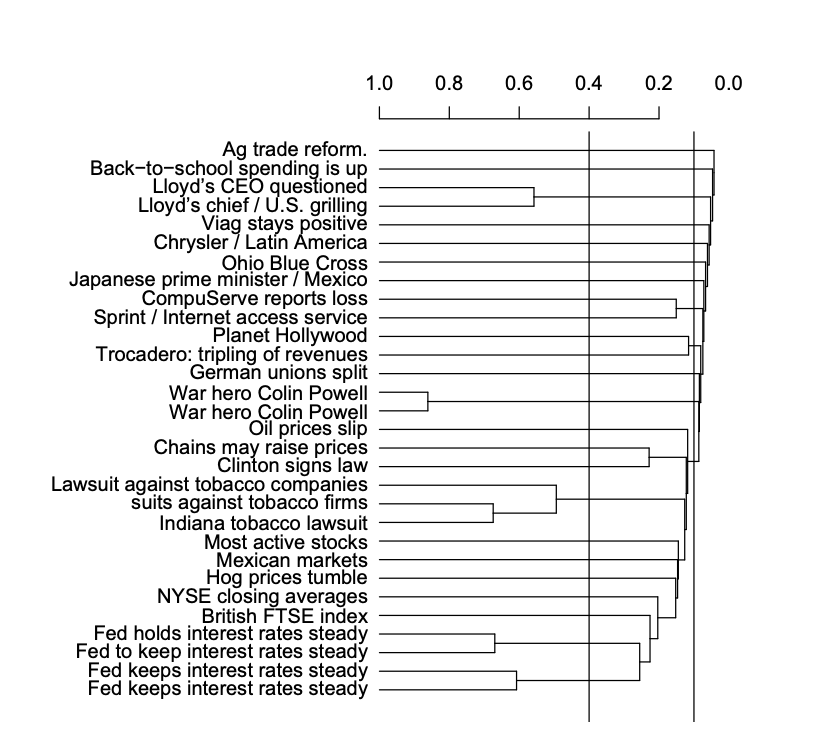
\includegraphics[width=0.5\textwidth]{dendrogram.png}
  \caption{Dendrogram of a single-linkage clustering of 30 documents from Reuters-RCV1. Two possible cuts of a dendrogram are shown: at 0.4 into 24 clusters and at 0.1 into 12 clusters.}
  \label{fig:dendrogram}
\end{figure}

A fundamental assumption in HAC is that the merge operation is monotonic, i.e., if \( s_1, s_2, ..., s_{K-1} \) are the combination similarities of the successive merges of an HAC, then \( s_1 \geq s_2 \geq ... \geq s_{K-1} \) holds. A non-monotonic hierarchical clustering contains at least one inversion \( s_i < s_{i+1} \) and contradicts the fundamental assumption that we chose the best merge available at each step. \\

\subsubsection{Linkage Criteria} The similarity between two clusters is defined as the linkage criteria. There are four common linkage criteria:
\begin{itemize}
    \item \textbf{Single Linkage:} The similarity between two clusters is defined as the similarity between the two most similar points in the two clusters.
    \item \textbf{Complete Linkage:} The similarity between two clusters is defined as the similarity between the two least similar points in the two clusters.
    \item \textbf{Average Linkage:} The similarity between two clusters is defined as the average similarity between all pairs of points in the two clusters.
    \item \textbf{Centroid Linkage:} The similarity between two clusters is defined as the similarity between the centroids of the two clusters. \\
\end{itemize}

\begin{figure}[h]
    \centering
    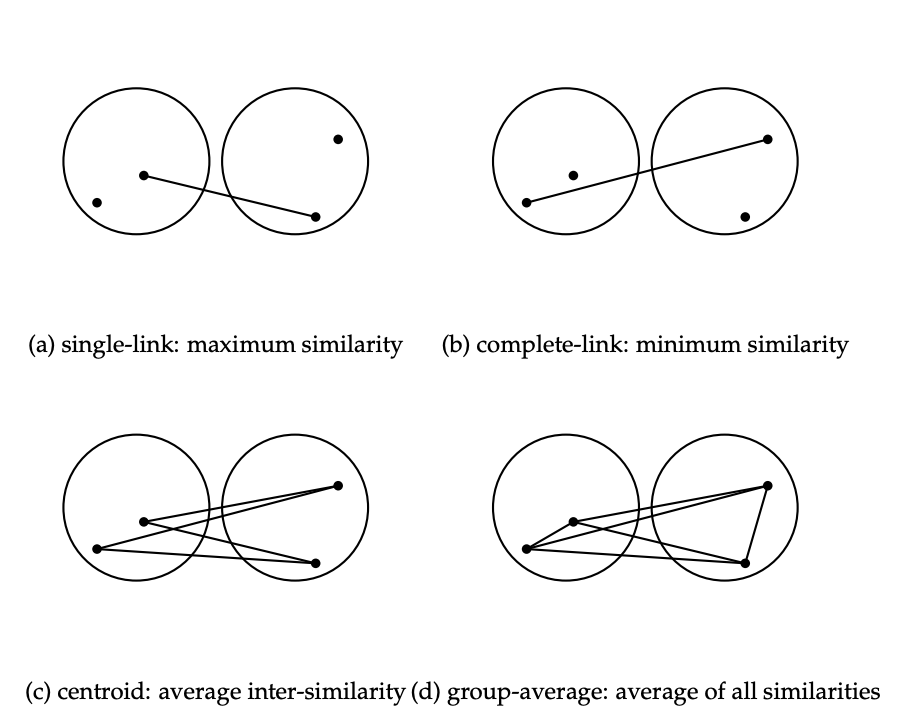
\includegraphics[width=0.5\textwidth]{linkage_criteria.png}
    \caption{Linkage criteria for hierarchical clustering.}
    \label{fig:linkage_criteria}
\end{figure}


As earlier mentioned, hierarchical clustering does not require a prespecified number of clusters, however, in some applications we want a partition of disjoint clusters just as in the case of flat clustering methods. How do we determine the number of clusters in a hierarchical clustering? A number of criteria can be used to determine the cutting point:
\begin{itemize}
    \item Cut at a prespecified level of similarity. For example, we cut the dendrogram at 0.4 if we want clusters with a minimum combination similarity of 0.4. In Figure~\ref{fig:dendrogram}, we can cut the dendrogram at 0.4 into 24 clusters or at 0.1 into 12 clusters.
    \item Cut the dendrogram where the gap between two successive combination similarities is largest. Such large gaps arguably indicate "natural" clusterings. Adding one more cluster decreases the quality of the clustering significantly, so cutting before this steep decrease occurs is desirable. 
    \item Apply equation \[ K = \underset{K'}{\text{argmin}} \left( RSS(K') + \lambda K' \right) \] where \( K' \) refers to the cut of the hierarchy that results in \( K' \) clusters, RSS is the residual sum of squares and \( \lambda \) is a penalty for each additional cluster. Instead of RSS, another measure of distortion can be used. 
    \item As in flat clustering, we can also prespecify the number of clusters \( K \) and select the cutting point that produces \( K \) clusters. \\
\end{itemize}




\textbf{Divisive Clustering}: Also known as the top-down approach. In Divisive Clustering, all of the data points are treated as one single cluster at the beginning, and a cluster hierarchy will be generated top-down. The cluster is split using a flat clustering algorithm. This procedure is applied recursively until each document is in its own singleton cluster. \\ 

Conceptually, divisive clustering is the reverse of agglomerative clustering and it is more complex because we need a second, flat clustering algorithm as a "subroutine". It has the advantage of being more efficient if we do not generate a complete hierarchy all the way down to individual document leaves. For a fixed number of top levels, using an efficient flat algorithm like K-means, top-down algorithms are linear in the number of documents and clusters. So they run much faster than HAC algorithms, which are at least quadratic. \\

There is evidence that divisive clustering produces better and more accurate results than bottom-up algorithms in some circumstances. Bottom-up methods make clustering decisions based on local patterns without initially taking into account the global distribution. These early decisions cannot be undone. Top-down clustering benefits from the complete information about the global distribution when making top-level partitioning decisions. \\

\subsection{DBSCAN (Density-Based Spatial Clustering of Applications with Noise)}
DBSCAN is a density-based clustering algorithm that groups together points that are closely packed together, based on a distance measure \cite{ester1996dbscan}. It is a popular algorithm for clustering because it does not require the number of clusters to be specified in advance, and it can find arbitrarily shaped clusters. \\

\begin{figure}[h]
    \centering
    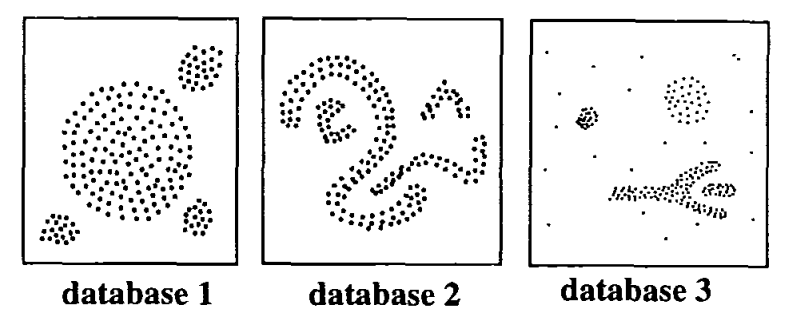
\includegraphics[width=0.5\textwidth]{dbscan_ds.png}
    \caption{Sample datasets with arbitrary shapes.}
    \label{fig:dbscan}
\end{figure}

The main reason why the algorithm recognises the clusters is that within each cluster we have a typical density of points which considerably higher than outside of the cluster. Furthermore, the density within the areas of noise is lower than the density within the areas of noise is lower than the density in any of the clusters. Note that the algorithm apply as well to 2D or 3D Euclidean space as to some high dimensional feature space. \\

The key idea is that for each point of a cluster the neighborhood of a given radius has to contain at least a minimum number of points, i.e., the density in the neighborhood has to exceed some threshold. The shape of a neighborhood is determined by the choice of a distance function for two points \( p \) and \( q \), denoted by \( d(p, q) \). For instance, when using Manhatten distance in 2D space, the shape of the neighborhood is rectangular. Note, that our approach works with any distance function so that an appropriate function can be chosen for some given application. For the purpose of proper visualization, all examples will be in 2D space using the Euclidean distance. \\

The hyperparamters of the algorithm are:
\begin{itemize}
    \item \( \epsilon \): Eps-neighborhood of a point \( p \) is defined as the set of all points within a distance of \( \epsilon \) from \( p \).
    \item \( MinPts \): Minimum number of points in an eps-neighborhood.
\end{itemize}

\subsubsection{Algorithm}
To find a cluster, DBSCAN starts with an artbitrary point \( p \) and retrieves all points density-reachable from \( p \) wrt. \( \epsilon \) and \( MinPts \). If \( p \) is a core point, this procedure yields a cluster wrt. \( \epsilon \) and \( MinPts \). If \( p \) is a border point, no points are density-reachable from \( p \) and DBSCAN visits the next point of the dataset. \\

Since the algorithm uses global values for \( \epsilon \) and \( MinPts \),  DBSCAN may merge two clusters into one cluster, if two clusters of different density are "close" to each other. Let the \textit{distance between two sets of points \( S_1 \) and \( S_2 \)} be defined as \( dist(S_1, S_2) = \min_{p \in S_1, q \in S_2} d(p, q) \). Then, two sets of points having at least the density of the thinnest cluster will be separated from each other only if the distance between the two sets is larger than \( \epsilon \). Consequently, a recursive call of DBSCAN may be necessary for the detected clusters with a higher value for \( MinPts \). This is however, no disadvantage because the recursive application of DBSCAN yields an elegant and very efficient basic algorithm. Furthermore, the recursive clustering of the points of a cluster is only necessary under conditions that can be easily detected. \\

If two clusters \( C_1 \) and \( C_2 \) are very close to each other, it might happen that some point \( p \) belongs to both \( C_1 \) and \( C_2 \). Then \( p \) must be border point in both clusters because otherwise \( C_1 \) would be equal to \( C_2 \) since we use global parameters. In this case, point \( p \) will be assigned to the clusters discovered first. Except from these rare situations, the result of DBSCAN is independent of the order in which the points of the dataset are visited. \\

\subsubsection{Determining the Parameters (\( \epsilon \) and \( MinPts \))}

In this section, we will discuss a simple but effective heuristic to determine the parameters \( \epsilon \) and \( MinPts \) of the "thinnest" cluster in the database. This heuristic is based on the following observation. Let \( d \) be the distance of a point \( p \) to its \( k \)-th nearest neighbor, then the \( d \)-neighborhood of \( p \) contains exactly \( k + 1 \) points for almost all points \( p \). The \( d \)-neighborhood of \( p \) contains more than \( k + 1 \) points only if several points have exactly the same distance d from p which is quite unlikely. Furthermore, changing \( l \) for a point in a cluster does not result in large changes of \( d \). This only happends if the \( k \)-th nearest neighbors of \( p \) for \( k = 1, 2, 3, ... \) are located approximately on a straight line which is in general not true for a point in a cluster. \\

For a given \( k \), a function \( k-dist \) from the database \( D \) to the real numbers, mapping each point to the distance from its \( k \)-th nearest neighbor. When sorting the points of the dataset in descending order of their \( k-dist \) values, the graph of this function gives some hints concerning the density distribution in the dataset. The graph is called \( sorted k-dist \) graph. If we choose an arbitrary point \( p \), set the parameter \( \epsilon \) to \( k-dist(p) \) and set the parameter \( Minpts \) to \( k \), all points with an equal or smaller \( k-dist \) value wil be core points. If we could find a \textit{threshold point} with the maximal \( k-dist \) value in the 
thinnest cluster of \( D \) we would have the desired parameter values. The threshold point is the first point in the first "valley" of the sorted k-dist graph. All points with a higher k-dist value (left of the threshold) are considered to be noise, all other points (right of the threshold) are assigned to some cluster. \\

\begin{figure}[h]
    \centering
    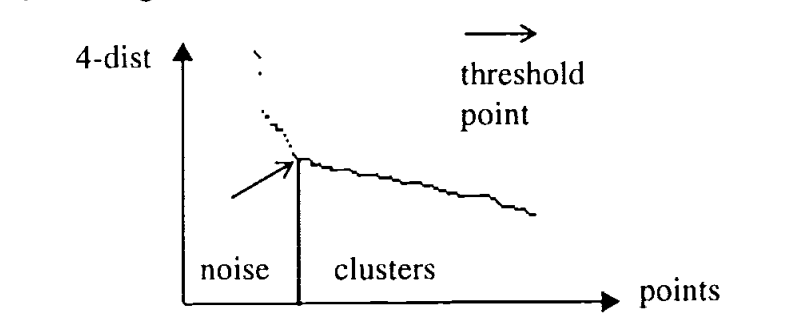
\includegraphics[width=0.5\textwidth]{4_dist_graph.png}
    \caption{Sorted 4-dist graph for sample dataset 3.}
    \label{fig:4_dist_graph}
\end{figure}

In general, it is very difficult to detect the first "valley" automatically, but it is relatively simple for a user to see this valley in a graphical representation. Therefore, we propose to follow an interative approach for determining the threshold point. \\

DBSCAN needs two parameter, \( \epsilon \) and \( MinPts \). However, our experiments indicate that the k-dist graphs for k > 4 do not significantly differ from the 4-dist graph and further, they need considerably more computation. Threrefore, we eliminiate the parameter \( MinPts \) by setting it to 4 for all datasets (for 2-dimensional data). We propose the following interactive approach for determining the parameter \( \epsilon \) of DBSCAN: 

\begin{enumerate}
    \item The system computes and displays the 4-dist graph for the dataset.
    \item If the user can estimate the percentage of noise, this percentage is entered and the system derives a proposal for the threshold point from it.
    \item The user either accepts the proposed threshold or selects another point as the threshold point. The 4-dist value of the threshold point is used as the \( \epsilon \) value for DBSCAN. 
\end{enumerate}


\subsection{Evaluation Metrics}
To assess the quality of clustering results, several evaluation metrics are used. These metrics help determine how well the algorithm has grouped similar data points and separated dissimilar ones. Evaluation can be divided into internal and external metrics. \\

\textbf{Internal Metrics:} These metrics are used to evaluate the quality of the clustering without reference to external information. They are based on the properties of the clusters themselves, such as the within-cluster similarity and the between-cluster separation. \\

\begin{figure}[h]
    \centering
    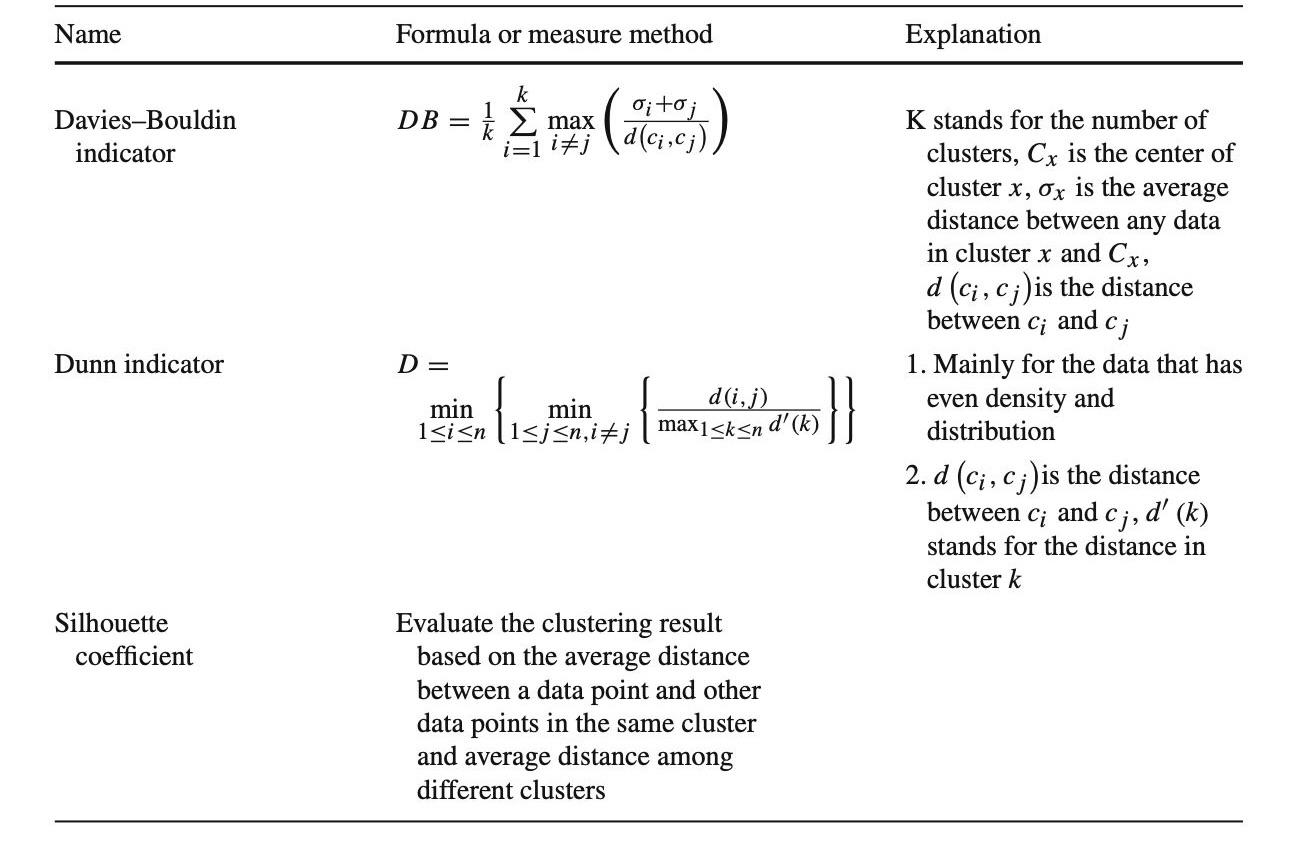
\includegraphics[width=0.5\textwidth]{internal_eval.png}
    \caption{Internal evaluation metrics \cite{saxena2017clustering}.}
    \label{fig:internal_eval}
\end{figure}


\textbf{External Metrics:} These metrics are used to evaluate the quality of the clustering with reference to external information. They are based on the properties of the clusters themselves, such as the within-cluster similarity and the between-cluster separation. \\

\begin{figure}[h]
    \centering
    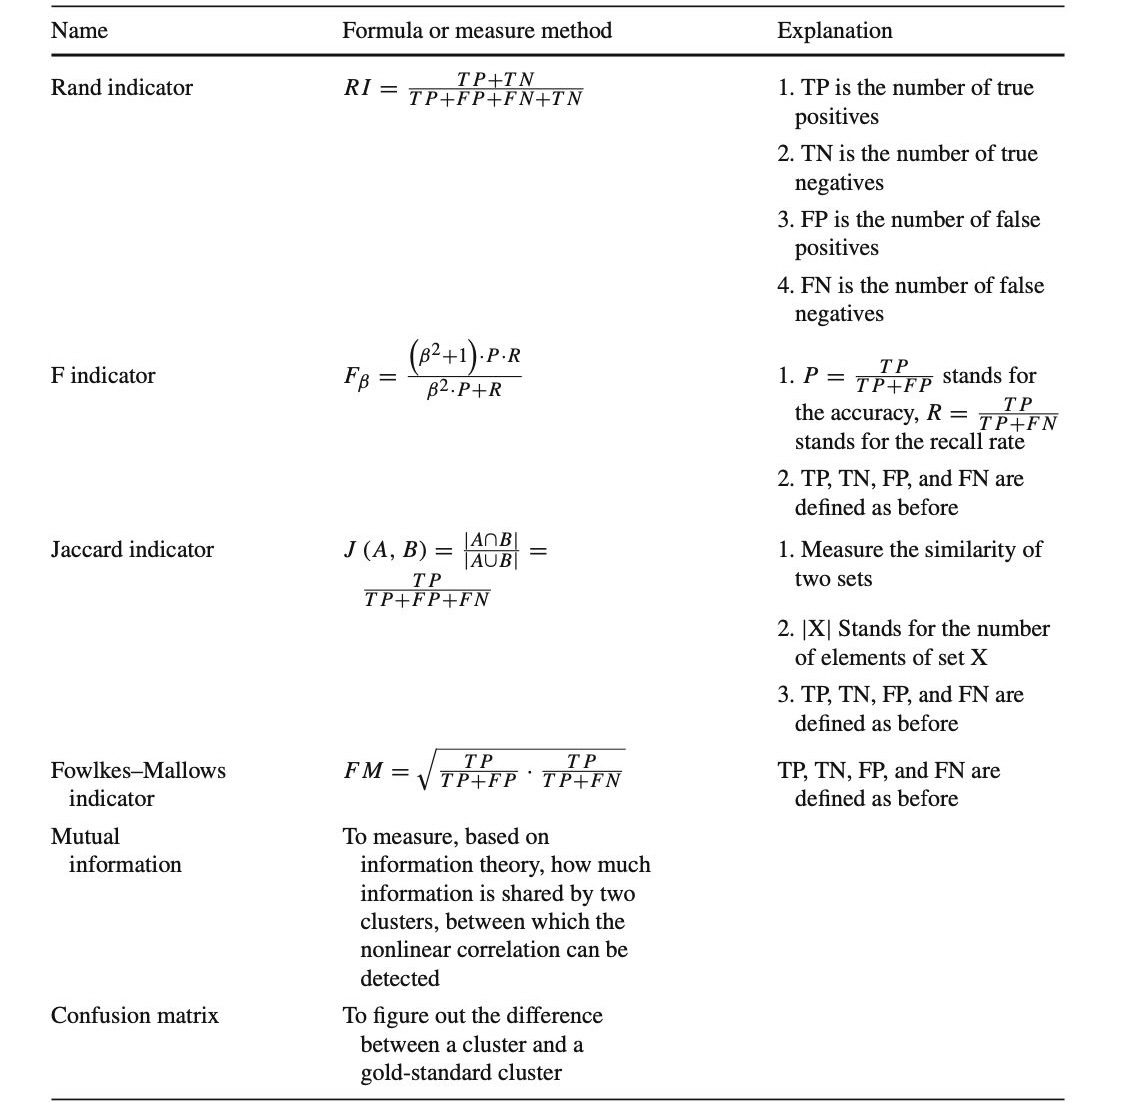
\includegraphics[width=0.5\textwidth]{external_eval.png}
    \caption{External evaluation metrics \cite{saxena2017clustering}.}
    \label{fig:external_eval}
\end{figure}

\section{Association Rule Learning}

Association rule learning is a rule-based learning method for discovering interesting relations between variables in large datasets \cite{agrawal1993mining}. It aims to identify strong rules discovered in databases using measures of interestingness such as support, confidence, and lift. \\

The main key concepts of association rule learning are:
\begin{itemize}
    \item \textbf{Itemset:} A collection of one or more items.
    \item \textbf{Support:} The support of a rule is the proportion of transactions that contain all the items in the rule.
    \item \textbf{Confidence:} The confidence of a rule is the proportion of transactions that contain all the items in the rule, divided by the proportion of transactions that contain the antecedent of the rule.
    \item \textbf{Lift:} The lift of a rule is the ratio of the confidence of the rule to the expected confidence of the rule if the antecedent and consequent were independent.
\end{itemize}


\subsection{Apriori Algorithm}
The Apriori algorithm is a popular algorithm for mining frequent itemsets and generating association rules \cite{agrawal1994fast}. It is based on the Apriori principle, which states that if an itemset is frequent, then all of its subsets must also be frequent. \\

Apriori is the first association rule mining algorithm that prioneered the use of support-based pruning to systematically control the exponential growth of candidate itemsets. \\

\begin{figure}[h]
    \centering
    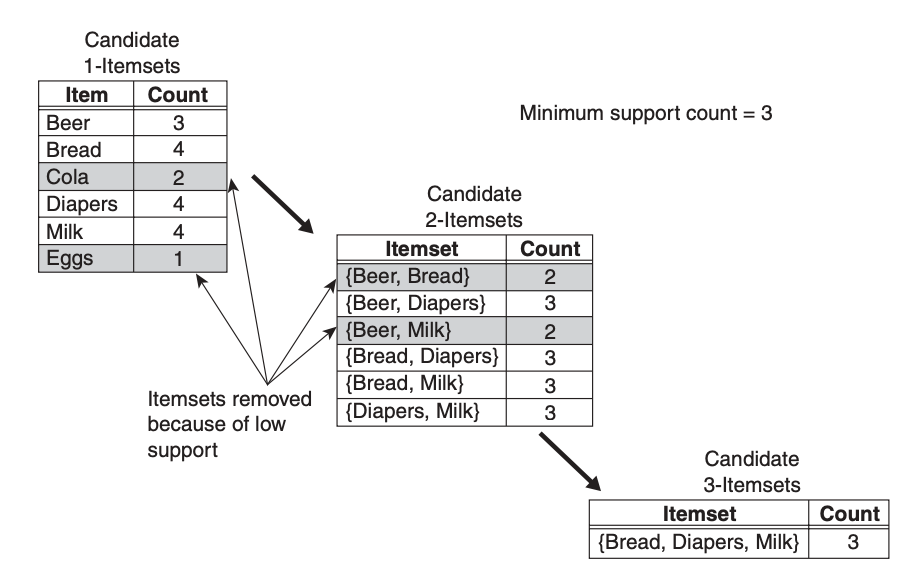
\includegraphics[width=0.5\textwidth]{apriori_algo.png}
    \caption{High-level illustration of the frequent itemset generation part of the Apriori algorithm.}
    \label{fig:apriori_algo}
\end{figure}

Initially, eveery item is considered as a candidate 1-itemset. After counting their supports, the candidate itemsets \( {Cola} \) and \( {Eggs} \) are discarded because they appear in fewer than three transactions. In the next iteration, candidate 2-itemsets are generated using only the frequent 1itemsets because the Apriori principle ensures that all the supersets of the infrequent 1-itemsets must be infrequent. because there are only four frequent 1-itemsets, the number of candidate 2-itemsets generated by the algorithm is 6. Two of these six candidates, 
\( {Beer, Bread} \) and \( {Beer, Milk} \) are subsequently found to be infrequent after computing their support values. The remaining four candidates are frequent, and thus will be used to generate candidate 3-itemsets. Without support-based pruning, there are 20 candidate 3-itemsets that can be formed using the six items given in this example. With the Apriori principle, we only need to keep candidate 3-itemsets whose subsets are frequent. The only candidate that has this property is \( {Bread, Diapers, Milk} \). \\

The effectiveness of the Apriori pruning strategy can be shown by counting the number of candidate itemsets generated. A brute-force strategy of enumerating all itemsets (up to size 3) as candidates will produce 

\[
\binom{6}{1} + \binom{6}{2} + \binom{6}{3} = 6 + 15 + 20 = 41
\]

candidates. With the Apriori principle, this number decreases to

\[
\binom{6}{1} + \binom{4}{2} + 1 = 6 + 6 + 1 = 13
\] 

candidates, which represents a 68\% reduction in the number of candidate itemsets even in this simple example. \\

\subsubsection{Algorithm}
Let \( C_k \) denote the set of candidate k-itemsets and \( F_k \) denote the set of frequent k-itemsets. The algorithm works as follows:

\begin{itemize}
    \item The algorithm initially makes a single pass over the data set to determine the support of each item. Upon completion of this step, the set of all frequent 1-itemsets, \( F_1 \), will be known (steps 1 and 2).
    
    \item Next, the algorithm will iteratively generate new candidate \( k \)-itemsets using the frequent \( (k-1) \)-itemsets found in the previous iteration (step 5). Candidate generation is implemented using a function called apriori-gen, which is described in Section 6.2.3.
    
    \item To count the support of the candidates, the algorithm needs to make an additional pass over the data set (steps 6–10). The subset function is used to determine all the candidate itemsets in \( C_k \) that are contained in each transaction \( t \). The implementation of this function is described in Section 6.2.4.
    
    \item After counting their supports, the algorithm eliminates all candidate itemsets whose support counts are less than \( minsup \) (step 12).
    
    \item The algorithm terminates when there are no new frequent itemsets generated, i.e., \( F_k = \emptyset \). \\
\end{itemize}

The frequent itemset generation part of the Apriori algorithm has two important characteristics. First, it is a \textbf{level-wise} algorithm; i.e., it traverses the itemset lattice one level at a time, from frequent 1-itemsets to the maximum size of frequent itemsets. Second, it employs a \textbf{generate-and-test} strategy for finding frequent itemsets. At each iteration, new candidate itemsets are generated from the frequent itemsets found in the previous iteration. The support for each candidate is then counted and tested against the \( minsup \) threshold. The total number of iterations needed by the algorithm is \( k_{max} + 1 \), where \( k_{max} \) is the maximum size of the frequent itemsets.


\subsection{Additional approaches}
There are several other approaches to association rule learning. They are as follows:

\subsubsection{FP-Growth Algorithm}
FP-Growth avoids Apriori’s expensive candidate generation by building a compact data structure called an FP-tree. It compresses the dataset by storing frequent patterns in a tree format and recursively mines the tree to find frequent itemsets, making it much faster and more scalable for large datasets.

\subsubsection{Eclat Algorithm}
Eclat uses a vertical data layout, representing items with lists of transaction IDs. It finds frequent itemsets by intersecting these ID lists, which is very efficient, especially on dense data, because it avoids generating large numbers of candidates explicitly.

\subsubsection{FP Max Algorithm}
FPMax is designed to find maximal frequent itemsets, which are the largest itemsets meeting the minimum support threshold without any frequent supersets. This approach reduces the number of patterns returned, simplifying the output without losing important information about the data’s structure.

\section{Real World Applications}

Some of the real world applications for unsupervised learning methods are:

\subsection{Dimensionality Reduction}
\begin{itemize}
    \item Data visualization: Reducing high-dimensional data to 2D or 3D (e.g. t-SNE, PCA) for exploratory analysis.
    
    \item Noise reduction: Removing irrelevant features in signal processing or images.
    
    \item Feature extraction for machine learning: Improving model training by reducing overfitting and computation.
    
    \item Genomics: Simplifying gene expression data for biomarker discovery.
\end{itemize}

\subsection{Clustering}
\begin{itemize}
    \item Customer segmentation: Marketers group customers based on purchasing behavior to tailor promotions.
    
    \item Image segmentation: Grouping pixels into regions for object recognition.
    
    \item Document clustering: Grouping news articles or search results by topic for easier navigation.
    
    \item Anomaly detection: Identifying fraud or network intrusions by spotting outlier clusters.
\end{itemize}

\subsection{Association Rule Learning}
\begin{itemize}
    \item Market basket analysis: Retailers find products frequently bought together (e.g. diapers and beer).
    
    \item Cross-selling strategies: Banks identify which financial products are bought together to target offers.
    
    \item Web usage mining: Understanding navigation patterns to improve site design and recommendations.
    
    \item Medical diagnosis: Discovering symptom–disease relationships in patient records.
\end{itemize}

\section{Conclusion}

Unsupervised learning remains a cornerstone of modern machine learning, offering tools to uncover hidden structures in data without the need for labeled examples. Its core techniques—dimensionality reduction, clustering, and association rule mining—serve as essential building blocks in fields ranging from healthcare and finance to supply chain optimization and recommender systems. \\

While traditional methods dominate due to their simplicity and interpretability, there is growing interest in more advanced approaches like autoencoders and generative models and hybrid approaches like self-supervised learning. Nevertheless, many real-world applications still favor robust and readily available algorithms from open-source libraries. \\

The increasing volume of unstructured and unlabeled data presents a clear need for scalable and interpretable unsupervised models. However, challenges such as model evaluation, lack of ground truth, and sensitivity to hyperparameters persist. \\
% Responsible use of unsupervised learning involves understanding its assumptions and limitations, and carefully validating results, especially when deployed in high-stakes domains. \\

This report has provided a foundational overview of key unsupervised methods, their mathematical formulations, and practical applications. As the field continues to evolve, future research should focus not only on algorithmic innovation but also on integration with domain knowledge, ethical deployment, and benchmarking frameworks to guide the selection of appropriate methods for real-world problems.

% Future directions in unsupervised learning include more interpretable models, hybrid approaches like self-supervised learning, and greater focus on fairness and privacy. As these methods mature, they will continue to shift how we understand and interact with data, particularly in domains where labeled information is scarce or expensive to obtain.


\section*{Author Contributions}
Laiba was responsible for designing the overall structure of the report and contributed to writing the Abstract, Section 1 (Introduction), Section 2, Section 3 (Dimensionality Reduction), and Section 4 (Clustering — K-Means only) and Section 7 (Conclusion). 

Nasrul contributed by completing Section 4 with additional clustering methods (Hierarchical Clustering, DBSCAN, and evaluation metrics), and by writing Section 5 (Association Rule Learning) and Section 6 (Real-World Applications).




% conference papers do not normally have an appendix


% use section* for acknowledgment
% \section*{Acknowledgment}


% The authors would like to thank...





% trigger a \newpage just before the given reference
% number - used to balance the columns on the last page
% adjust value as needed - may need to be readjusted if
% the document is modified later
%\IEEEtriggeratref{8}
% The "triggered" command can be changed if desired:
%\IEEEtriggercmd{\enlargethispage{-5in}}

% references section

% can use a bibliography generated by BibTeX as a .bbl file
% BibTeX documentation can be easily obtained at:
% http://mirror.ctan.org/biblio/bibtex/contrib/doc/
% The IEEEtran BibTeX style support page is at:
% http://www.michaelshell.org/tex/ieeetran/bibtex/
%\bibliographystyle{IEEEtran}
% argument is your BibTeX string definitions and bibliography database(s)
%\bibliography{IEEEabrv,../bib/paper}
%
% <OR> manually copy in the resultant .bbl file
% set second argument of \begin to the number of references
% (used to reserve space for the reference number labels box)
\bibliographystyle{IEEEtran}
\bibliography{references}
% \begin{thebibliography}{1}

% \bibitem{IEEEhowto:kopka}
% H.~Kopka and P.~W. Daly, \emph{A Guide to \LaTeX}, 3rd~ed.\hskip 1em plus
%   0.5em minus 0.4em\relax Harlow, England: Addison-Wesley, 1999.
% \bibitem{zhu2005semi}
% X.~Zhu, ``Semi-Supervised Learning Literature Survey,'' \emph{Computer Sciences Technical Report 1530}, University of Wisconsin-Madison, 2005.
% intro-article

% \end{thebibliography}




% that's all folks
\end{document}


